{If $f$ and $g$ are functions whose graphs are shown, evaluate the expressions.\\
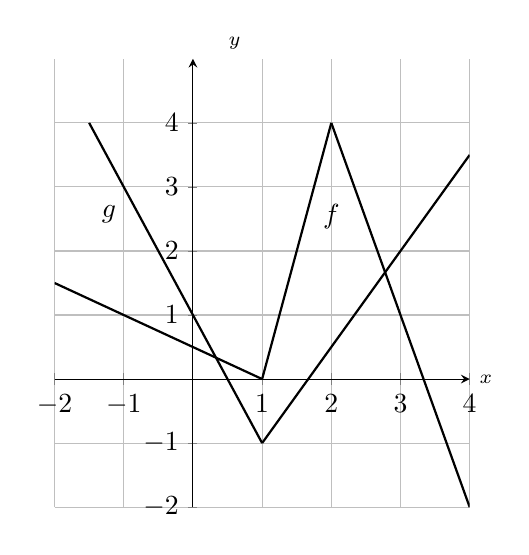
\begin{tikzpicture}
\begin{axis}[axis y line=middle,axis x line=middle, ymajorgrids=true, xmajorgrids=true, ymin=-2,ymax=5, xmin=-2,xmax=4, name=myplot, xscale=1/1.3, ytick={-2,-1,0,1,2,3,4}]
\addplot [{\colorone}, domain=-1.5:1,thick] {-2*x+1}; 
\addplot [{\colorone}, domain=1:4,thick] {1.5*x-2.5};
\addplot [{\colortwo}, domain=-2:1, thick] {-.5*x+.5};
\node[label={30:{$g$}}] at (axis cs:-1.6,2.2) {};
\addplot [{\colortwo}, domain=1:2, thick] {4*x-4};
\node[label={30:{$f$}}] at (axis cs:1.6,2.1) {};
\addplot [{\colortwo}, domain=2:4, thick] {-3*x+10};
\end{axis}
\node [right] at (myplot.right of origin) {\scriptsize $x$};
\node [above] at (myplot.above origin) {\scriptsize $y$};
\end{tikzpicture}\\
(a) $(fg)'(-1)$  \quad (b) $(f/g)'(-1)$ \\
(c) $(fg)'(3)$ \quad (d) $(g/f)'(3)$}
{(a) $-\frac{7}{2}$ (b) $\frac{1}{8}$ (c) $-\frac{9}{2}$ (d) $\frac{15}{2}$}
